%%%%%%%%%%%%%%%%%%%%%%%%%%%%%%%%%%%%%%%%%%%%%%%%%%%%%%%%%%%%%%%%%%%%%%%%%%%
%% This file is part of the book
%%
%% Algorithmic Graph Theory
%% http://code.google.com/p/graph-theory-algorithms-book/
%%
%% Copyright (C) 2009, 2010, 2011 Minh Van Nguyen <nguyenminh2@gmail.com>
%%
%% See the file COPYING for copying conditions.
%%%%%%%%%%%%%%%%%%%%%%%%%%%%%%%%%%%%%%%%%%%%%%%%%%%%%%%%%%%%%%%%%%%%%%%%%%%

\documentclass{article}

\usepackage{tikz}
\usetikzlibrary{external}
\usetikzlibrary{trees}
\tikzexternalize{expression-tree-perfect-square}

\begin{document}

\begin{figure}
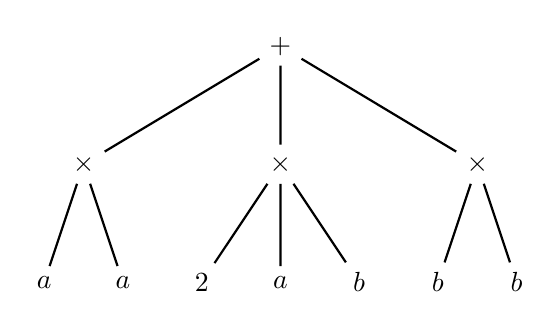
\begin{tikzpicture}
[-,thick]
\node {$+$}
  [sibling distance=2.5cm]
  child {node {$\times$}
    [sibling distance=1cm]
    child {node {$a$}}
    child {node {$a$}}
  }
  child {node {$\times$}
    [sibling distance=1cm]
    child {node {$2$}}
    child {node {$a$}}
    child {node {$b$}}
  }
  child {node {$\times$}
    [sibling distance=1cm]
    child {node {$b$}}
    child {node {$b$}}
  };
\end{tikzpicture}
\end{figure}

\end{document}
